\chapter{Układ zamka}
\label{chap:controller}

    Niniejszy rozdział przedstawia zagadnienia związane z procesem implementacji układu zamka. Uzasadnia wybór wykorzystanych w projekcie technologii sprzętowych i programowych, opisuje sposób konfiguracji środowiska deweloperskiego, a także przedstawia wybrane problemy implementacyjne.

    \section{Wykorzystane technologie}

        \subsection{Mikrokontroler}

            Istotnym problemem natury implementacyjnej jest wybór odpowiedniego mikrokontrolera, który spełni wymagania dotyczące wydajności energetycznej oraz bezpieczeństwa systemu, jednocześnie zapewniając możliwość obsługi kilku układów peryferyjnych i wsparcie dla komunikacji bezprzewodowej, a także wygodne i elastyczne środowisko deweloperskie.

            Spośród wielu rozwiązań dostępnych na rynku wybrany został mikrokontroler ESP32. Oprócz wszystkich wymienionych wyżej cech, charakteryzuje się on możliwością przetwarzania równoległego za pomocą dwóch fizycznych rdzeni, co otwiera nowe możliwości w kwestii projektowania i implementacji oprogramowania, szczególnie w przypadku istnienia rygorystycznych wymagań dotyczących czasu odpowiedzi układu. Zapewnia sprzętowe wsparcie dla algorytmów kryptograficznych oraz możliwość zaawansowanej kontroli pracy podzespołów w zakresie zasilania, a także umożliwia komunikację z peryferiami za pośrednictwem programowalnych wejść/wyjść GPIO (ang. \textit{General-Purpose Input/Output}). \textbf{Napisać jakie ma currenty}

            Oprogramowanie dla mikrokontrolera ESP32 może być wytwarzane w środowisku Arduino IDE lub z wykorzystaniem oficjalnej platformy programistycznej Espressif IoT Development Framework (ESP-IDF) firmy Espressif Systems. ESP-IDF opiera się na systemie FreeRTOS (ang. \textit{Free Real-Time Operating System}, system operacyjny czasu rzeczywistego), w wersji 8.2.0, port Xtensa~\cite{esp-idf-freertos-smp-changes}. Ze względu na chęć uzyskania pełniejszej kontroli nad mikrokontrolerem zdecydowano się na użycie w projekcie platformy ESP-IDF.

        \subsection{Czytnik RFID}

            Głównym kryterium wyboru czytnika identyfikatorów RFID jest prostota integracji z mikrokontrolerem. Ze względu na fakt, iż jego zasilaniem zarządzać będzie mikrokontroler, niski pobór mocy nie stanowi kryterium przesądzającego. Wybrano układ MFRC522 produkowany przez firmę NXP Semiconductors. Układ obsługuje urządzenia o częstotliwości nośnej 13,56 MHz oraz umożliwia komunikację poprzez protokół SPI (ang. \textit{Serial Peripheral Interface}).

        \subsection{Czujnik ruchu}

            Czujnik ruchu posiada krytyczne znaczenie w układzie zamka. Jako jedyny z podzespołów musi być zasilany przez cały czas pracy układu. Ze względu na wymaganie wykorzystania zasilania bateryjnego w układzie istotną cechą jest jak najniższy pobór mocy w stanie spoczynku. Wybranym rozwiązaniem jest czujnik PIR (ang. \textit{Passive Infra Red}, pasywny czujnik podczerwieni), model HC-SR501. Wykrycie obiektu sygnalizowane jest stanem wysokim na cyfrowym wyjściu. Czujnik HC-SR501 wyposażony jest w dwa potencjometry umożliwiające regulację czasu trwania stanu wysokiego po wykryciu obiektu oraz czułości czujnika. Układ posiada także zworkę, którą można samodzielnie zlutować i w ten sposób wybrać jeden z dwóch możliwych trybów:

            \begin{itemize}
                \item Tryb \textit{repeatable} - po wykryciu obiektu stan wysoki utrzymywany jest przez określony przez potencjometr czas,
                \item Tryb \textit{non-repeatable} - stan wysoki po wykryciu obiektu utrzymywany jest przez cały czas występowania ruchu. Po zatrzymaniu ruchu stan wysoki utrzymywany jest przez określony przez potencjometr czas.
            \end{itemize}

            Dzięki temu możliwe jest dobranie parametrów czujnika w taki sposób, aby użytkownik był wykrywany w odpowiednim momencie, co przekłada się na bardziej optymalne działanie układu.

            \textbf{Napisać jak u nas są te parametry ustawione}

            \textbf{Napisać jaki ma zasięg, sprzeczne źródła :/}

            \textbf{TBD - schemat jak sa polaczone pinami te wszystkie komponenty}

            \textbf{TBD - opisać układ do zasilania czytnika RFID}

    \section{Konfiguracja środowiska}

        Platforma programistyczna ESP-IDF zapewnia zestaw narzędzi (ang. \textit{toolchain}) umożliwiających wytwarzanie oprogramowania dla mikrokontrolera ESP32. Pobranie ESP-IDF sprowadza się do sklonowania repozytorium. Platforma ESP-IDF nie jest częścią projektu, lecz samodzielnym modułem linkowanym do projektu za pomocą zmiennej środowiskowej.

        Komponenty potrzebne do wytwarzania oprogramowania dla ESP32 z użyciem ESP-IDF oraz sam proces w uproszczeniu przedstawia rysunek \ref{fig:esp32_dev} \cite{esp-idf-get-started}.

        \begin{figure}[]
            \centering
            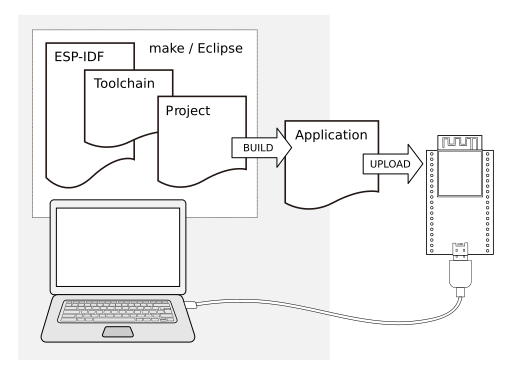
\includegraphics[width=\textwidth]{chapters/images/esp32_dev.png}
            \caption{Wytwarzanie oprogramowania dla ESP32}
            \label{fig:esp32_dev}
        \end{figure}

        Konfiguracja, budowanie i \textbf{flashowanie jak to powiedziec po polsku} aplikacji odbywa się za pomocą dedykowanego skryptu dostarczanego przez platformę.

    \section{Oprogramowanie mikrokontrolera}

        \subsection{Komponenty}

            ESP-IDF umożliwia podział aplikacji na komponenty oraz ich łatwą konfigurację w procesie kompilacji za pomocą tekstowego menu. Jak wyjaśnia \cite{esp-idf-build-system}, komponenty to modularne i samodzielne fragmenty kodu kompilowane do bibliotek statycznych i linkowane do aplikacji. Niektóre z nich są dostarczane przez platformę ESP-IDF. Istnieje też możliwość tworzenia własnych komponentów.

            Kod źródłowy oprogramowania mikrokontrolera został podzielony na cztery komponenty:

            \begin{enumerate}
                \item Komponent główny (\textit{main}),
                \item Komponent RFID,
                \item Komponent WiFi,
                \item Komponent sterujący (\textit{flow-controller}).
            \end{enumerate}

            \textbf{Napisac ktore rzeczy sa konfigurowalne przez menuconfig}

        \subsection{Współbieżność}

            Jak opisuje \cite{esp-idf-freertos-smp-changes}, oryginalny system FreeRTOS został zaprojektowany z myślą o przetwarzaniu za pomocą jednego rdzenia. ESP32 posiada jednak dwa rdzenie o wspólnej pamięci, co pozwala na przemienne wykonywanie zadań na obu rdzeniach. Koncepcja zadań (ang. \textit{tasks}) istniejąca w oryginalnym FreeRTOS w ESP-IDF została zmodyfikowana na potrzeby wsparcia mikrokontrolera o dwóch rdzeniach oraz SMP (ang. \textit{symmetric multiprocessing}, symetryczne przetwarzanie wieloprocesorowe). Każde z zadań ma określony priorytet, na podstawie którego algorytm planowania ustala kolejność wykonywania. Dzieje się to indywidualnie dla każdego rdzenia, lecz lista zadań gotowych do wykonania jest pomiędzy nimi współdzielona.

            Aby maksymalnie wykorzystać możliwości platformy ESP-IDF w kwestii współbieżności jednocześnie unikając nadmiernego skompilowania kodu, zdecydowano się na wykorzystanie w ramach aplikacji dwóch zadań. Należy nadmienić, że przez większą część czasu mikrokontroler nie wykonuje operacji, których zrównoleglenie byłoby korzystne. Jedyną sytuacją, w której warto zastosować przetwarzanie współbieżne jest nawiązywanie połączenia z serwerem oraz odczyt danych z czytnika RFID. Obie czynności mogą okazać się czasochłonne. W aplikacji jednowątkowej, odczyt danych z czytnika RFID musiałby zakończyć się przed rozpoczęciem nawiązywania połączenia, lub odwrotnie. Jeśli zastosujemy zapewniany przez ESP-IDF mechanizm zadań, możemy wykonywać obie operacje jednocześnie.

            Do synchronizacji zadań wykorzystany został mechanizm tzw. \textit{event group} (grupy zdarzeń) dostarczany przez system FreeRTOS. Zakłada on wykorzystanie przez współpracujące zadania współdzielonej grupy zdarzeń, składającej się z zestawu flag, oraz udostępnia funkcje do operowania na niej. Możliwe operacje to ustawianie w stan wysoki lub niski danej flagi oraz oczekiwanie na stan wysoki flagi. Korzystny z perspektywy synchronizacji wątków jest fakt, że oczekiwanie na dane zdarzenie blokuje aktualnie wykonywane zadanie, umożliwiając oddanie sterowania innym oczekującym zadaniom.

            \textbf{Tutaj jakiś diagram pokazujący komunikację między taskami czy coś}

        \subsection{Stan głębokiego uśpienia}

            ESP32 oferuje efektywną i elastyczną technologię zarządzania energią. Dokument ~\cite{esp32-ds} wymienia pięć dostępnych stanów energetycznych:

            \begin{enumerate}
                \item \textit{Active mode}
                    Aktywne CPU wraz z układem radiowym.

                \item \textit{Modem-sleep mode}
                    Aktywne CPU, układ radiowy wyłączony.
                
                \item \textit{Light-sleep mode}
                    Uśpione CPU. Pamięć i peryferia RTC (ang. \textit{Real-Time Clock}, zegar czasu rzeczywistego) wraz z koprocesorem ULP (ang. \textit{Ultra Low Power co-processor}) są aktywne. Jakiekolwiek zdarzenia wybudzające doprowadzą do wybudzenia układu.

                \item \textit{Deep-sleep mode}
                    Tylko pamięć i peryferia RTC pozostają zasilone. Dane dotyczące połączeń WiFi i Bluetooth zostają przechowane w pamięci RTC. Opcjonalnie dostępny jest koprocesor ULP.

                \item \textit{Hibernation mode}
                    Wewnętrzny rezonator kwarcowy wraz z koprocesorem ULP zostają wyłączone. Również pamięć RTC jest wyłączona. Wybudzenie możliwe jest tylko poprzez timer RTC lub wejścia RTC GPIO.

            \end{enumerate}

            \textbf{Można dodać jakie są zużycia energii tutaj}

            Z punktu widzenia wymagań dotyczących poboru energii niezwykle przydatnym trybem jest tryb głębokiego uśpienia (ang. \textit{deep-sleep mode}). Dzięki jego wykorzystaniu możliwe jest przebywanie mikrokontrolera w trybie niskiego zużycia energii przez większą część czasu. Ze względu na cyfrowy charakter wyjścia czujnika ruchu, jako sposób wybudzenia mikrokontrolera skonfigurowano tryb EXT0 (ang. \textit{External Wakeup 0}, wybudzenie zewnętrzne) umożliwiający wykorzystanie modułu RTC IO (ang. \textit{Real-Time Clock Input Output}) w celu zainicjowania wybudzenia. Inne możliwe źródła wybudzenia to m.in. zegar RTC (ang. \textit{timer}) czy przerwanie wbudowanego czujnika dotykowego (ang. \textit{touch pad}). Konfiguracja trybu wybudzania odbywa się programowo jako jedna z pierwszych operacji aplikacji.

        \subsection{Biblioteka do zarządzania czytnikiem RFID}

            Do zarządzania czytnikiem MFRC522 wykorzystano zewnętrzną bibliotekę\footnote{Alija Bobija, \textit{C library for interfacing ESP32 with MFRC522 RFID card reader}, \url{https://github.com/abobija/esp-idf-rc522} (rewizja 557af67)}.

             % Inicjalizacja rozpoczyna się od inicjalizacji interfejsu SPI na określonych z góry wyjściach mikrokontrolera. Następnie rozpoczyna się cykliczne odpytywanie czytnika rc522 za pomocą wspomnianego interfejsu~\cite{esp-idf-rc522}. W przypadku sygnalizacji wykrycia karty przez czytnik, pozyskiwany jest numer karty, odpytywanie zostaje zakończone a numer karty zostaje przekazany do komponentu sterującego.

        \subsection{Przepływ sterowania}

            Przepływ sterowania w oprogramowaniu mikrokontrolera ukazują rysunki \ref{fig:flowchart1} i \ref{fig:flowchart4}. Na rysunkach \ref{fig:flowchart2} i \ref{fig:flowchart3} przedstawiono przepływ sterowania w zadaniach \textit{wifi} i \textit{rfid}. 

            \begin{figure}[]
                \centering
                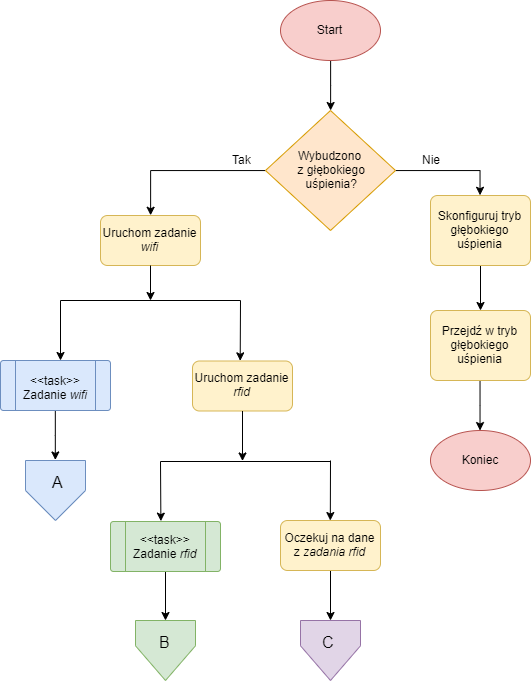
\includegraphics[width=\textwidth]{chapters/images/flowchart1.png}
                \caption{Schemat blokowy przepływu sterowania oprogramowania mikrokontrolera}
                \label{fig:flowchart1}
            \end{figure}

            \begin{figure}[]
                \centering
                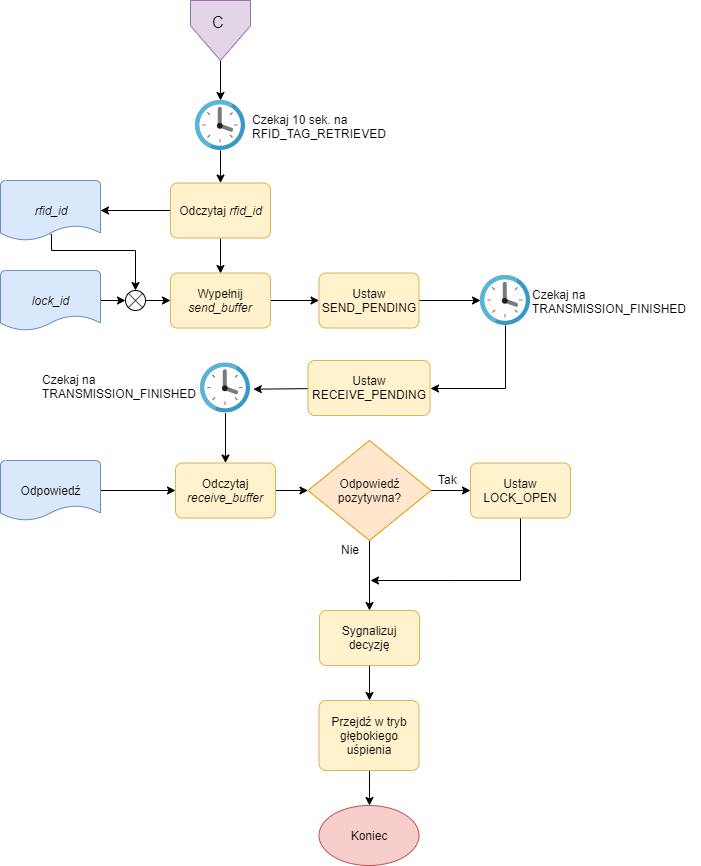
\includegraphics[width=\textwidth]{chapters/images/flowchart4.png}
                \caption{Schemat blokowy przepływu sterowania oprogramowania mikrokontrolera, c.d.}
                \label{fig:flowchart4}
            \end{figure}

            \begin{figure}[]
                \centering
                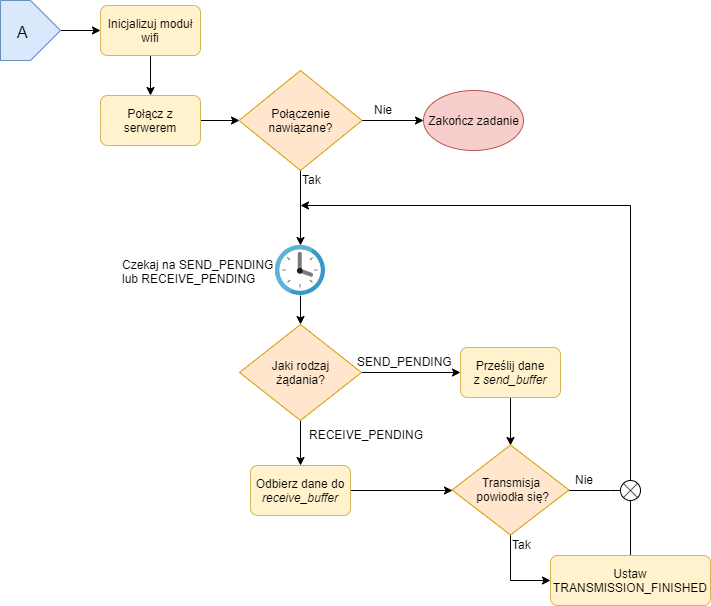
\includegraphics[width=\textwidth]{chapters/images/flowchart2.png}
                \caption{Schemat blokowy przepływu sterowania zadania obsługującego komunikację z serwerem}
                \label{fig:flowchart2}
            \end{figure}

            \begin{figure}[]
                \centering
                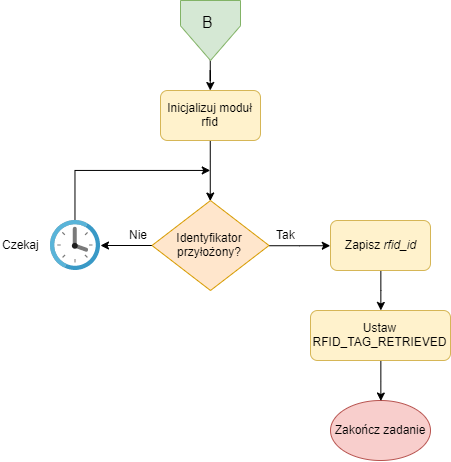
\includegraphics[width=0.8\textwidth]{chapters/images/flowchart3.png}
                \caption{Schemat blokowy przepływu sterowania zadania obsługującego czytnik RFID}
                \label{fig:flowchart3}
            \end{figure}




    %         \subsection{Współbieżność}
    %             Ze względu na restrykcyjne wymagania dotyczące czasu trwania procesu zestawiania połączenia z serwerem, wykorzystano przetwarzanie współbieżne na dwóch wątkach.

    %             \textbf{Diagram pokazujący jak taski między sobą się komunikują itd}

    %             Powiadamianie o wszystkich zdarzeniach w oprogramowaniu mikrokontrolera realizowane jest przez mechanizm tzw. \textit{Event Group}. Jest on zapewniany przez system FreeRTOS. W przypadku wystąpienia zdarzenia zostaje ono zapisane we wspomnianym wyżej \textit{Event Group}, co jest równoznaczne z ustawieniem w stan wysoki bitu przypisanego danemu zdarzeniu. Kluczowy z perspektywy przepływu sterowania jest wykorzystany mechanizm oczekiwania na zdarzenia, który przez wywłaszczenie oczekującego wątku pozwala na efektywną implementację synchronizacji wątków.

    %             \textbf{Dodać źródło dokumentacja FreeRTOS}

    %         \textbf{TBD - Przenieść część poniższych informacji na Schematy blokowe}

    %         \subsection{Pierwsze uruchomienie}

    %             Przy pierwszym uruchomienu zamka, które następuje automatycznie po podłączeniu zasilania do układu, wykonywana jest procedura przejścia w stan głębokiego uśpienia (Deep-sleep mode). W tym celu jako sposób wybudzenia konfigurowany jest tryb EXT0 (External Wakeup 0). Tryb ten wymusza aby po przejściu w stan uśpienia podtrzymane zostało zasilanie peryferiów RTC (ang. \textit{Real-Time Clock}, zegar czasu rzeczywistego)~\cite{esp32-api-ref-deep-sleep}, co z kolei pozwala na konfigurację źródła wybudzającego przerwania zewnętrznego jako wybranego wejścia RTC GPIO. W projekcie w tym celu wykorzystany został pin nr 26. Ze względu na charakterystykę wykorzystanego źródła przerwania (pasywny czujnik zbliżeniowy), konieczne było zastosowanie trybu pulldown dla wspomnianego wyżej wejścia aby zapobiec występowaniu na nim stanu nieokreślonego. Po konfiguracji źródła przerwania układ zostaje wprowadzony w stan uśpienia.

    %         \subsection{Wybudzenie z głębokiego uśpienia}

    %             \textbf{Podzielić blok tekstu na części bardziej skupiające się na poszczególnych komponentach - TBD}

    %             Po wykryciu ruchu, czujnik PIR generuje stan wysoki na linii wybudzającej mikrokontrolera, co wywołuje procedurę wyjścia z głębokiego uśpienia. Po wybudzeniu następuje inicjalizacja systemu obsługi zdarzeń, wykorzystywany przez wszystkie wątki jako główne narzędzie sygnalizacji postępu i synchronizacji dostępu do danych. Po przygotowaniu mechanizmu sygnalizacji zdarzeń komponent sterujący inicjuje współbieżną inicjalizację komponentów RFID oraz WiFi.

    %             Inicjalizacja komponentu WiFi może przebiec na dwa sposoby. Jeśli następuje po raz pierwszy od czasu podłączenia zasilania do układu, wymagane jest wykonanie konfiguracji sterownika WiFi dostarczanego przez ESP-IDF. W tym celu ustawiane są dane dostępu do sieci (SSID i hasło, osadzone w bezpośrednio w oprogramowaniu) a sterownik przestawiany jest w tryb station, pozwalający mikrokontrolerowi na nawiązanie połączenia z punktem dostępu sieci bezprzewodowej. Następnie dane konfiguracji zapisywane są w pamięci nieulotnej. Alternatywny scenariusz następuje przy każdej następnej inicjalizacji. Wykorzystuje on dane zapisane podczas poprzedniej inicjalizacji w celu odtworzenia konfiguracji sterownika WiFi.

    %             Wspomniana wyżej konfiguracja zostaje następnie wykorzystana do nawiązania połączenia z siecią bezprzewodową. Następnie następuje próba zestawienia bezpiecznego połączenia z serwerem, opartego na mechanizmach TLS i wzajemnego uwierzytelnienia (ang. \textit{Mutual authentication}). Po udanym zestawieniu połączenia z wykorzystaniem uścisku dłoni TLS (ang. \textit{TLS Handshake}) program przechodzi do pętli obsługi żądań transmisji pochodzących od pozostałych komponentów.

    %             Na listingu \ref{snip:wifi_client} przedstawiono pseudokod pętli obsługi żądań w komponencie WiFi.

    %             \textbf{Zmodyfikowac ten pseudokod, zeby byl bardziej czytelny i zrozumialy dla kogos nieznajacego wewnetrznej struktury i specyfiki kodu}
    %             \lstinputlisting[language=Python,label=snip:wifi_client,caption=Pseudokod pętli obsługi żądań w komponencie WiFi]{chapters/pseudocodes/wifi_client_pseudocode.py}

    %             Komponent RFID bazuje na zewnętrznej bibliotece~\cite{esp-idf-rc522}. Inicjalizacja rozpoczyna się od inicjalizacji interfejsu SPI na określonych z góry wyjściach mikrokontrolera. Następnie rozpoczyna się cykliczne odpytywanie czytnika rc522 za pomocą wspomnianego interfejsu~\cite{esp-idf-rc522}. W przypadku sygnalizacji wykrycia karty przez czytnik, pozyskiwany jest numer karty, odpytywanie zostaje zakończone a numer karty zostaje przekazany do komponentu sterującego. \textbf{TBD}

    %             \textbf{sterowanie po przylozeniu karty TBD}
    %             Po stworzeniu wątków odpowiedzialnych za wykonanie kodu komponentów WiFi i RFID komponent sterujący rozpoczyna oczekiwanie na sygnalizację wykrycia karty przez komponent RFID. Gdy to nastąpi, odczytany zostaje pozyskay numer karty. W celu wymiany danych z serwerem, wykorzystywany interfejs udostępniany przez komponent WiFi w postaci funkcji do transmisji wychodzącej i przychodzącej \textbf{dodac pseudokod funkcji żądania transmisji, uszczegółowić}. Zależnie od informacji zwrotnej od serwera, następuje przyznanie dostępu, lub jego odmowa i ponowne przejście w stan uśpienia.

    % \section {Wykorzystane technologie}

    %     \subsection{ESP32}

    %         ESP32-DevKitC jest produkowaną przez firmę Espressif platformą deweloperską bazującą na module ESP32-WROOM-32D. Sercem modułu jest układ z rodziny ESP32 (ESP32-D0WD) wyposażony w CPU (ang. \textit{Central Processing Unit}, centralna jednostka obliczeniowa) o dwóch rdzeniach, z których każdy może być kontrolowany niezależnie~\cite{esp32-wroom32-ds}. Moduł integruje Bluetooth, Bluetooth Low Energy oraz WiFi, a także szeroki zakres peryferiów: czujniki dotyku, czujniki pola magnetycznego, interfejs karty SD, Ethernet, SPI, UART (ang. \textit{Universal Asynchronous Receiver-Transmitter}), I\textsuperscript{2}S (ang. \textit{Inter-IC Sound}) i I\textsuperscript{2}C (ang. \textit{Inter-Integrated Circuit})~\cite{esp32-wroom32-ds}. Dodatkowo umożliwia korzystanie z niskoenergetycznego koprocesora Ultra-Low-Power (ang. \textit{ULP co-processor}), podczas gdy główne jednostki pozostają w trybie głębokiego uśpienia~\cite{esp32-tech-ref-man}.

    %         ESP32 oferuje efektywną i elastyczną technologię zarządzania energią. Dokument \textit{ESP32 Series Datasheet} wymienia pięć predefiniowanychstanów energetycznych~\cite{esp32-ds}:
    %         \begin{enumerate}
    %             \item Active mode: Aktywne CPU wraz z układem radiowym, możliwa bezprzewodowa transmisja.
    %             \item Modem-sleep mode: Aktywne CPU z konfigurowalnym zegarem. Chip radiowy w tym trybie pozostaje wyłączony.
    %             \item Light-sleep mode: Uśpione CPU. Pamięć i peryferia RTC wraz z koprocesorem ULP pozostają aktywne. Jakiekolwiek zdarzenia wybudzające (MAC, host, timer RTC i zewnętrzne przerwania) doprowadzą do wybudzenia układu.
    %             \item Deep-sleep mode: Tylko pamięć RTC i peryferia RTC pozostają zasilone. Dane dotyczące połączeń WiFi i Bluetooth zostają przechowane w pamięci RTC. Opcjonalnie dostępny jest koprocesor ULP.
    %             \item Hibernation mode: Wewnętrzny rezonator kwarcowy o częstotliwośći 8~MHz wraz z koprocesorem ULP zostają wyłączone. Również pamięć RTC jest wyłączona. Wybodzenie możliwe jest tylko poprzez timer RTC lub predefiniowane wejścia RTC GPIO.
    %         \end{enumerate}
    %         Jest to szczególnie istotne z punktu widzenia wymagań dotyczących poboru energii.

    %     \subsection{Czytnik MFRC522}

    %         Do realizacji komunikacji w standardzie RFID High Frequency (13,56~MHz) wykorzystany został zintegrowany odbiornik/nadajnik MFRC522 produkowany przez firmę NXP Semiconductors, umożliwający bezprzewodową komunikację z kartami zgodnymi ze standardem ISO/IEC 14443 A/MIFARE. Układ wspiera komunikację poprzez interfejsy SPI, UART oraz I\textsuperscript{2}C~\cite{mfrc522-ds}.

    %     \subsection{Czujnik zbliżeniowy}
    %         \textbf{TBD}

    % \section{Bezpieczeństwo}

    %     \textbf{Tutaj opisać mechanizmy wykorzystane w celu zapewnienia bezpieczeństwa systemu - TBD}

    %     Ważnym aspektem opracowanego systemu jest bezpieczeństwo. Bezpieczeństwo systemu tworzą następujące składowe:
    %         \begin{enumerate}
    %             \item Bezpieczeństwo zastosowanego mikrokontrolera
    %             \item Bezpieczeństwo komunikacji bezprzewodowej
    %             \item Bezpieczeństwo serwera
    %         \end{enumerate}

    %         \subsection{Bezpieczeństwo mikrokontrolerów}
    %             \textbf{TBD}

    %         \subsection{Bezpieczeństwo komunikacji bezprzewodowej}
    %             \textbf{TBD}

    %         \subsection{Bezpieczeństwo serwera}
    %             \textbf{TBD}


    % \section{Problemy}

    %     Konfiguracja WiFi?
    %     Sygnalizacja stanu baterii?
    %     zarządzanie stanami energetycznymi
    %     Enkrypcja flash

    %     \subsection{Zarządzanie energią}

    %         \textbf{Szacunki długości życia na baterii - TBD}
    %         \textbf{Teoretyczne zużycie podawane w specyfikacji komponentów}
    %         \textbf{Pomiary poboru mocy w różnych fazach działania - TBD}